\chapter{Kooperacyjne planowanie tras}
\label{ch:cooperative_pathfinding}

% \section{Metody planowania tras}
Spośród metod wykorzystywanych do kooperacyjnego planowania tras dla wielu robotów można wyróżnić dwie zasadnicze grupy \cite{latombe}:
\begin{itemize}
	\item {\bf Zcentralizowane} - drogi wyznaczane są dla wszystkich agentów na raz (jednocześnie). Metody tego typu są często trudne do zrealizowania (gdyż do rozwiązania jest złożony problem optymalizacyjny) oraz mają bardzo dużą złożoność obliczeniową ze względu na ogromną przestrzeń przeszukiwania. Struktura organizacyjna jest scentralizowana - decyzje podejmowane są na podstawie centralnego systemu.
	\item {\bf Rozproszone} (ang. {\it decoupled} lub {\it distributed}) - podejście to dekomponuje zadanie na niezależne lub zależne w niewielkim stopniu problemy dla każdego agenta. Dla każdego robota droga wyznaczana jest osobno, w określonej kolejności, następnie rozwiązywane są konflikty (kolizje dróg).
	Zastosowanie metod rozproszonych wiąże się najczęściej z koniecznością przydzielania priorytetów robotom, co stanowi istotny problem, gdyż od ich wyboru może zależeć zupełność algorytmu. Nie należy mylić tej metody z zagadnieniem typu {\it Non-Cooperative Pathfinding}, w którym agenci nie mają wiedzy na temat pozostałych planów i muszą przewidywać przyszłe ruchy pozostałych robotów \cite{cooppath}. W podejściu rozproszonym agenci mają pełną informację na temat stanu pozostałych robotów, lecz wyznaczanie dróg odbywa się w określonej kolejności.
\end{itemize}

W systemach czasu rzeczywistego istotne jest, aby rozwiązanie problemu planowania tras uzyskać w krótkim, deterministycznym czasie, dlatego w tego typu systemach chętniej używane są techniki rozproszone.

\section{Metoda pól potencjałowych}
Metoda pól potencjałowych (ang. {\it Artificial Potential Field} lub {\it Potential Field Technique}) polega na zastosowaniu zasad oddziaływania między ładunkami znanych z elektrostatyki. Roboty i przeszkody traktowane są jako ładunki jednoimienne, przez co "odpychają się" siłą odwrotnie proporcjonalną do kwadratu odległości (dzięki temu unikają kolizji między sobą). Natomiast punkt docelowy robota jest odwzorowany jako ładunek o przeciwnym biegunie, przez co robot jest "przyciągany" do celu.
Główną zasadę działania metody przedstawiono na rysunku \ref{fig:image_potentialfield}.

Technika ta jest bardzo prosta i nie wymaga wykonywania złożonych obliczeń (w odróżnieniu do pozostałych metod zcentralizowanych).
Niestety bardzo powszechny jest problem osiągania minimum lokalnego, w którym suma wektorów daje zerową siłę wypadkową. Robot zostaje "uwięziony" w takim minimum lokalnym, przez co nie jest w stanie dotrzeć do wyznaczonego celu. Do omijania tego problemu muszą być stosowane inne dodatkowe metody \cite{potentialfield}.
Metoda pól potencjałowych nie daje gwarancji ani optymalności, ani nawet zupełności.
\begin{figure}
	\centering
	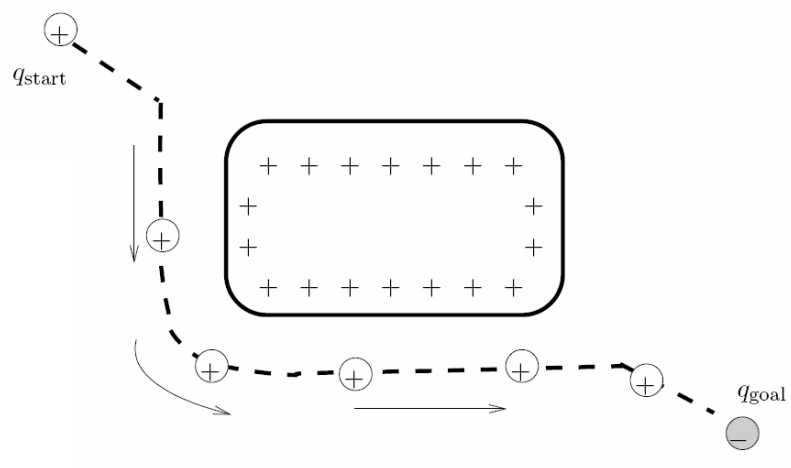
\includegraphics[width=12cm]{img/potential-field}
	\caption{Zasada działania metody pól potencjałowych. Dodatni ładunek $q_{start}$ reprezentuje robota. Przyciągany jest w stronę ujemnego ładunku celu $q_{goal}$, zaś odpychany jest od dodatnio naładowanej przeszkody. Źródło: \cite{howie_potentialfield}}
	\label{fig:image_potentialfield}
\end{figure}

\section{Rozproszone planowanie tras}
Najczęściej stosowanymi podejściami są metody oparte o algorytm A* lub jego pochodne.
W celu wykonywania wydajnych obliczeń w algorytmach przeszukujących grafy, nawet w przypadku ciągłej przestrzeni mapy, stosuje się podział na dyskretną siatkę pól (por. rys. \ref{fig:img_games_warcraft-map-editor}) \cite{hierpathfindinginrts}.

\begin{figure}[H]
	\centering
	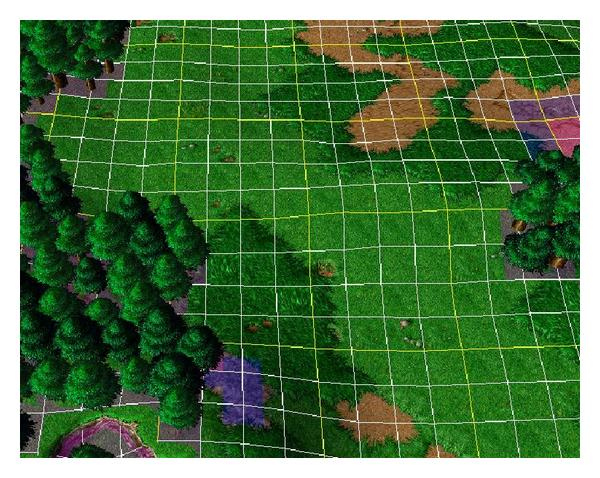
\includegraphics[width=7cm]{img/games/warcraft-map-editor}
	\caption{Ciągła przestrzeń mapy zdyskretyzowana do siatki pól. \\ Źródło: edytor map z gry Warcraft III.}
	\label{fig:img_games_warcraft-map-editor}
\end{figure}

Popularne podejścia unikające planowania w wysoko wymiarowej zbiorowej przestrzeni konfiguracyjnej to techniki rozproszone i uwzględniające priorytety \cite{optpriorities}.
Pomimo, że metody te są bardzo efektywne, mają dwie główne wady:
\vspace{-0.5em}
\begin{itemize}[itemsep=0em]
	\item Nie są zupełne - nie dają gwarancji znalezienia rozwiązania, nawet gdy takie istnieje.
	\item Wynikowe rozwiązania mogą być nieoptymalne.
\end{itemize}

% TODO-MGR
% W artykule \cite{optpriorities} przedstawione zostało podejście do optymalizowania układu priorytetów dla rozproszonych i uwzględniających priorytety technik planowania.
% Proponowana metoda wykonuje randomizowane przeszukiwanie z techniką hill-climbing do znalezienia rozwiązania i do skrócenia całkowitej długości ścieżek.
% Technika ta została zaimplemenotwana i przetestowana na prawdziwych robotach oraz w rozległych testach symulacyjnych, dając zadowalające rezultaty.

\section{Planowanie uwzględniające priorytety}
Często używaną w praktyce metodą jest planowanie z uwzględnianiem priorytetów. 
W tej technice agenci otrzymują unikalne priorytety. Algorytm wykonuje indywidualne planowanie sekwencyjnie dla każdego agenta w kolejności od najwyższego priorytetu. Trajektorie agentów o wyższych priorytetach są ograniczeniami (ruchomymi przeszkodami) dla pozostałych agentów \cite{async_decentralized_spacetime_cp}.

Złożoność ogólnego algorytmu rośnie liniowo wraz z liczbą agentów, dzięki temu to podejście ma zastosowanie w problemach z dużą liczbą agentów.
Algorytm ten jest zachłanny i niezupełny w takim znaczeniu, że agentów zadowala pierwsza znaleziona trajektoria niekolidująca z agentami wyższych priorytetów. 

Istotną rolę doboru priorytetów robotów w procesie planowania tras ukazuje prosty przykład przedstawiony na rysunku \ref{fig:image_article1_fig1}. Jeśli robot 1 (zmierzający z punktu S1 do G1) otrzyma wyższy priorytet niż robot 2 (zmierzający z S2 do G2), spowoduje to zablokowanie przejazdu dla robota 2 i w efekcie prawidłowe, istniejące rozwiązanie nie zostanie znalezione.
\begin{figure}
	\centering
	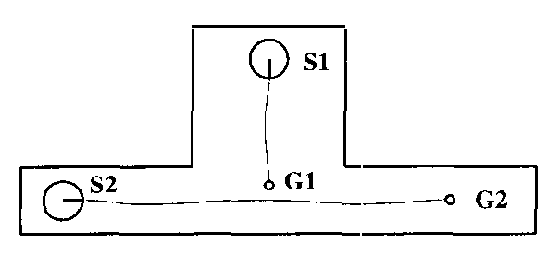
\includegraphics[width=6cm]{img/article1/fig1}
	\caption{Sytuacja, w której żadne rozwiązanie nie zostanie znalezione, stosując planowanie uwzględniające priorytety, jeśli robot 1 ma wyższy priorytet niż robot 2. Źródło: \cite{optpriorities}}
	\label{fig:image_article1_fig1}
\end{figure}

Układ priorytetów może mieć także wpływ na długość uzyskanych tras. Potwierdzający to przykład został przedstawiony na rysunku \ref{fig:image_article1_ppt6}. W zależności od wyboru priorytetów, wpływających na kolejność planowania tras, otrzymujemy różne rozwiązania.
\begin{figure}
	\centering
	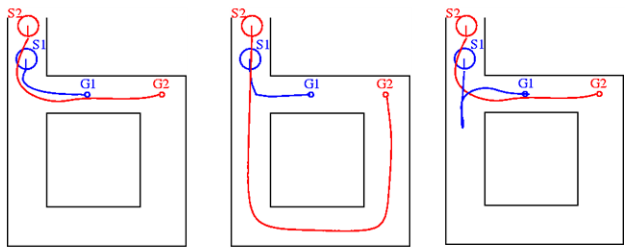
\includegraphics[width=13cm]{img/article1/ppt6}
	\caption{a) Niezależne planowanie optymalnych tras dla 2 robotów; b) suboptymalne rozwiązanie, gdy robot 1 ma wyższy priorytet; c) rozwiązanie, gdy robot 2 ma wyższy priorytet. Źródło: \cite{optpriorities}}
	\label{fig:image_article1_ppt6}
\end{figure}

\section{Metoda Path Coordination}
Jedną z metod rozproszonego planowania tras z uwzględnianiem priorytetów jest {\it Path Coordination}, której idea przedstawia się w następujących krokach \cite{optpriorities}:
\begin{enumerate}
	\item Wyznaczenie ścieżki dla każdego robota {\bf niezależnie} (np. za pomocą algorytmu A*)
	\item Przydział priorytetów
	\item Próba rozwiązania możliwych konfliktów między ścieżkami. Roboty utrzymywane są na ich indywidualnych ścieżkach (wyznaczonych na początku), wprowadzane modyfikacje pozwalają na zatrzymanie się, ruch naprzód, a nawet cofanie się, ale tylko {\bf wzdłuż trajektorii} w celu uniknięcia kolizji z robotem o wyższym priorytecie.
\end{enumerate}